\documentclass[tikz,border=8pt]{standalone}
\usepackage[T1]{fontenc}
\usetikzlibrary{arrows.meta,backgrounds,shapes.geometric}
\definecolor{ink}{HTML}{24343C}
\definecolor{teal}{HTML}{247B79}
\definecolor{coral}{HTML}{AE5B47}

% Adapted from the user's sandbox/pic.tex for a standalone documentation figure.
% Edge plan: source -> target | meaning | corridor.
% clauses -> sat | propositional input | central forward row.
% sat -> assignment | candidate assignment | central forward row.
% assignment -> theory | mapped theory literals | central forward row.
% theory -> done | consistent assignment | short right exit.
% sat -> unsat | Boolean contradiction | upper terminal band.
% theory -> lemma | theory conflict | lower right band.
% lemma -> sat | exclude inconsistent assignment | lower feedback band.
% The lazy loop is explanatory; Primo also has callbacks during SAT search.
% Unknown/unsupported outcomes and model construction are omitted here.

\begin{document}
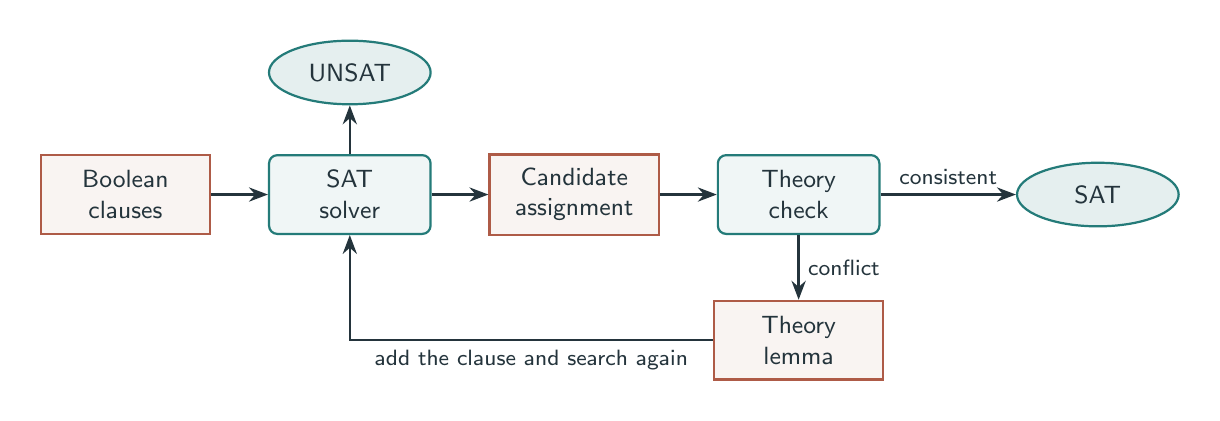
\begin{tikzpicture}[
  font=\sffamily\small, text=ink,
  every node/.style={align=center, inner sep=5pt},
  process/.style={draw=teal, fill=teal!7, rounded corners=3pt,
    text width=1.7cm, minimum height=1.0cm, line width=0.8pt},
  artifact/.style={draw=coral, fill=coral!7,
    text width=1.8cm, minimum height=1.0cm, line width=0.8pt},
  terminal/.style={draw=teal, fill=teal!12, ellipse,
    text width=1.1cm, minimum height=0.7cm, line width=0.8pt},
  flow/.style={-{Stealth[length=2.4mm]}, draw=ink, line width=0.9pt},
  label/.style={font=\sffamily\footnotesize, inner sep=3pt},
  background rectangle/.style={fill=white}, show background rectangle
]
  \node[artifact] (clauses) at (0,0) {Boolean\\clauses};
  \node[process] (sat) at (2.85,0) {SAT\\solver};
  \node[artifact] (assignment) at (5.7,0) {Candidate\\assignment};
  \node[process] (theory) at (8.55,0) {Theory\\check};
  \node[terminal] (done) at (12.35,0) {SAT};
  \node[terminal] (unsat) at (2.85,1.55) {UNSAT};
  \node[artifact] (lemma) at (8.55,-1.85) {Theory\\lemma};

  \draw[flow] (clauses.east) -- (sat.west);
  \draw[flow] (sat.east) -- (assignment.west);
  \draw[flow] (assignment.east) -- (theory.west);
  \draw[flow] (theory.east) -- node[label, above] {consistent} (done.west);
  \draw[flow] (sat.north) -- (unsat.south);
  \draw[flow] (theory.south) -- node[label, right] {conflict} (lemma.north);
  \draw[flow] (lemma.west) -- node[label, below] {add the clause and search again}
    (2.85,-1.85) -- (sat.south);
\end{tikzpicture}
\end{document}
